\documentclass[%
12pt, %
final, % 
oneside, % 
onecolumn, %  
centertags]{article} % относится к классу article и размер шрифта 12 пунктовб, {article: статья, report: отчеты и диссертации, book: книга, letter: письмо}

% \usepackage{fontspec}
 
% \setmainfont{Times New Roman}

% \documentclass[a4paper, 12pt]{report}

\topmargin= -30pt % насколько сверху будет страница
\textheight= 650pt


\usepackage[utf8]{inputenc} % задает кодировку, utf-8 кодировка, включающая в себя знаки почти всех языков мира
\usepackage[english]{babel} % подключает необходимые языки, основным языком является английский

\selectlanguage{english} % настройки будут на английском, но писать будет на русском

\usepackage{euscript}
\usepackage{supertabular}

\renewcommand{\baselinestretch}{1.0} 

\usepackage[colorlinks=true,linkcolor=blue,unicode=true,urlcolor = blue]{hyperref} %hypered
\usepackage[pdftex]{graphicx} % для графики

\usepackage{amsthm, amssymb, amsmath, amsfonts} % математический пакет, математические шрифты
\usepackage{textcomp}
\usepackage[noend]{algorithmic}
\usepackage[ruled]{algorithm}
\usepackage{lipsum}
\usepackage{indentfirst}
\usepackage{babel}
\usepackage{pgfplots}
\usepackage{setspace}
\usepackage{xcolor}
\usepackage{hyperref}
\usepackage{subfigure}

\setcounter{secnumdepth}{5}
\setcounter{tocdepth}{5}
\newcommand\simpleparagraph[1]{%
  \stepcounter{paragraph}\paragraph*{\theparagraph\quad{}#1}}
\usepackage{listings}
% \usepackage{xcolor}
%\usepackage{minted}

\lstset { %
     language=C++,
     backgroundcolor=\color{black!5}, % set backgroundcolor
     basicstyle=\footnotesize,% basic font setting
}


\linespread{1.0} 
\setlength{\parindent}{2.4em}
\setlength{\parskip}{0.1em}

\pgfplotsset{compat=1.9}
\pgfplotsset{model/.style = {blue, samples = 100}} 
\pgfplotsset{experiment/.style = {red}}

\theoremstyle{plain}
\binoppenalty=10000

\newtheorem{theorem}{Theorem}[section] % theorem

\theoremstyle{definition}
% \newtheorem{definition}{Определение}[subsection]
\newtheorem{definition}{Definition}[subsection]

\theoremstyle{remark}
% \newtheorem{remark}{Замечание}[section]

% \newtheorem{corollary}{Следствие}

% \newtheorem{proposition}{Proposition}

% \newtheorem{example}{Пример}

% \newtheorem{lemma}{Лемма}[section]

\renewcommand*{\proofname}{Proof}

\graphicspath{ {./images/} }


% \usepackage{amsmath,amsfonts,amssymb, setspace}  % Разнообразные математические команды и значки
% \usepackage{indentfirst}     % Отступ в первом абзаце

% \pagestyle{empty}
\usepackage[left=2.5cm, right=1.5cm, top=2.5cm, bottom=2.5cm]{geometry}
\usepackage[medium]{titlesec}
\usepackage{graphicx}
% \graphicspath{ {./images/} }

\begin{document}

	\begin{titlepage} 
		\begin{center}
		\textbf{}\\[2.0cm]
		\LARGE FEDERAL STATE AUTONOMOUS EDUCATIONAL INSTITUTION OF HIGHER EDUCATION \\[0.5cm]
		\Large ITMO UNIVERSITY \\[3cm]
		\LARGE Report\\
		\Large OpenMP. Practical tasks No. $1-3$. \\
		\Large Parallel algorithms for the analysis and synthesis of data \\[4cm]


		\begin{flushright}
		Performed by\\
		Aleksandr Shirokov\\
		J4133c\\
		Accepted by\\
		Petr Andriushchenko
		\end{flushright}

		\vfill 

		{\Large {St. Petersburg}} \par
		{\Large {2021}}
		\end{center} 
	\end{titlepage}

\tableofcontents
\newpage


\section{Assignments}

\subsection{Assignment 3.}

\subsubsection{Formulation of the problem}

Compile and run \textsc{Assignment3.c} program. Explain in detail how it works.

\subsubsection{Example of launch parameters and output. Detailed description of solution}

Code for \textbf{assignment 3} is \href{https:\//github.com/aptmess/parallel_algorithms/blob/master/HT/hw_mpi/Assignment3.c}{here}.

Compilation example: \textsc{mpic++ -o ./cpf/3.o Assignment3.c}

Launch example:

\begin{itemize}
	\item Not in parallel: \textsc{./cpf/3.o}

	\begin{center}
		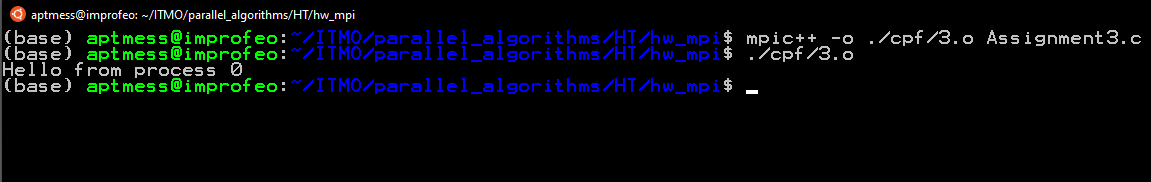
\includegraphics[scale=0.5]{3.1.png}
	\end{center}


	\item In parallel: \textsc{mpirun --oversubscribe -np 4 ./cpf/3.o} (have a problem without \textsc{--oversubscribe} option.

	\begin{center}
		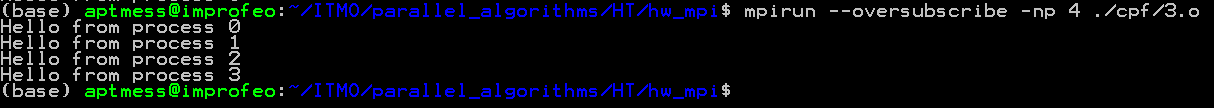
\includegraphics[scale=0.5]{3.2.png}
	\end{center}

\end{itemize}

Let's move to the the code and explain how it works.

\begin{center}
		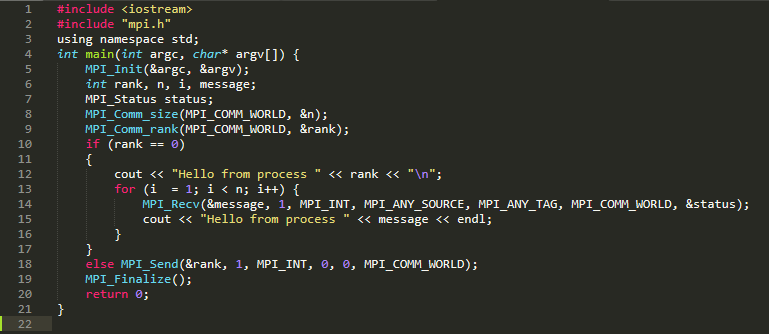
\includegraphics[scale=0.75]{3.code.png}

		Assignment3 code
\end{center}

\begin{enumerate}
	\item Line 5 - \textsc{MPI\_Init} - initialisation, starting the parallel part with arguments of main function;
	\item Line 6 - initialize variables, especially \textit{rank} for rank of process and \textit{n} for amount of process
	\item Line 7 - creating \textsc{MPI\_status}, variable status contains three attibutes of message:
	\begin{itemize}
		\item \textsc{MPI\_source} - number of the sending process;
		\item \textsc{MPI\_tag} - name of text message, identifier;
		\item \textsc{MPI\_error} - error code.
	\end{itemize}
	\item Line 7 - getting number of processes (\textit{n} varialbe)
	\item Line 8 - getting rank of the process (\textit{rank} variable)
	\item Line 10 - \textsc{if} statement
	\begin{itemize}
		\item \textsc{if rank == 0} - then we are printing 'Hello from process 0' and in range $i=[1..10]$ where $i$ is number of process, waiting for incoming messages from any source (who is quicklier will be write earlier) with any tag using syntax of function \textsc{MPI\_Send}. The information 'Hello from process \%message' is printing after we get message on each iteration of cycle.
		\item else - from processes with rank not $0$ sending messages to process with rank $0$. The message contains information about processes's rank.
	\end{itemize}
	\item Line 19 - Ending parallel part
\end{enumerate}

I have analysed the first code with mpi, explain how it works, compile it and show results.



\subsection{Appendix}

The link to the sourse code which is placed on my \href{https://github.com/aptmess/parallel_algorithms}{github}.


\end{document}